\documentclass[11pt,a4paper]{article}

\usepackage[margin=1.5cm]{geometry}
\usepackage{graphicx}
\usepackage{amsmath}
\usepackage{amssymb}
\usepackage{listings}
\usepackage{xcolor}
\usepackage{hyperref}
\usepackage{tikz}
\usetikzlibrary{shapes.multipart, positioning, arrows.meta}
\usepackage{booktabs}
\usepackage{caption}

% Hyperlink configuration
\hypersetup{
    colorlinks=true,
    linkcolor=blue,
    filecolor=magenta,      
    urlcolor=blue,
    pdftitle={IRE 460 - Lab Report 01: Digital Wallet Backend System},
    pdfauthor={Shahriar Alom Masud}
}

% Dart syntax highlighting configuration
\definecolor{codegreen}{rgb}{0,0.55,0}
\definecolor{codegray}{rgb}{0.45,0.45,0.45}
\definecolor{codepurple}{rgb}{0.55,0,0.75}
\definecolor{backcolour}{rgb}{0.98,0.98,0.98}
\definecolor{keywordblue}{rgb}{0.0,0.2,0.8}

\lstdefinelanguage{Dart}{
  morekeywords={abstract,as,assert,async,await,break,case,catch,class,const,continue,default,deferred,do,dynamic,else,enum,export,extends,extension,external,factory,false,final,finally,for,Function,get,hide,if,implements,import,in,interface,is,late,library,mixin,new,null,of,on,operator,part,rethrow,return,set,show,static,super,switch,sync,this,throw,true,try,typedef,var,void,while,with,yield},
  sensitive=true,
  morecomment=[l]{//},
  morecomment=[s]{/*}{*/},
  morestring=[b]",
  morestring=[b]'
}

\lstdefinestyle{dartstyle}{
    language=Dart,
    backgroundcolor=\color{backcolour},   
    commentstyle=\color{codegreen}\itshape,
    keywordstyle=\color{keywordblue}\bfseries,
    numberstyle=\tiny\color{codegray},
    stringstyle=\color{codepurple},
    basicstyle=\ttfamily\scriptsize\linespread{0.88}\selectfont,
    breaklines=true,                 
    numbers=left,                    
    numbersep=5pt,                  
    tabsize=2,
    frame=single,
    rulecolor=\color{lightgray},
    showspaces=false,
    showstringspaces=false,
    showtabs=false
}

\lstset{style=dartstyle}

\begin{document}

% ==============================================================================
% COVER PAGE (PAGE 1)
% ==============================================================================
\begin{titlepage}
    \begin{tikzpicture}[remember picture, overlay]
        \draw[line width=1.2pt] 
            ([shift={(1.2cm,-1.2cm)}]current page.north west) 
            rectangle 
            ([shift={(-1.2cm,1.2cm)}]current page.south east);
        \draw[line width=0.5pt] 
            ([shift={(1.32cm,-1.32cm)}]current page.north west) 
            rectangle 
            ([shift={(-1.32cm,1.32cm)}]current page.south east);
    \end{tikzpicture}

    \centering
    \vspace*{0.4cm}

    
\includegraphics[width=3.6cm]{screenshots/uftb_logo.png}\\[0.4cm]
    {\normalsize \textbf{UNIVERSITY OF FRONTIER TECHNOLOGY, BANGLADESH}}\\[0.16cm]
    {\footnotesize \textbf{DEPARTMENT OF INTERNET OF THINGS AND ROBOTICS ENGINEERING (IRE)}}\\[0.14cm]
    {\footnotesize FACULTY OF CYBER PHYSICAL SYSTEM ENGINEERING}\\[0.55cm]

    \noindent\rule{0.88\textwidth}{0.85pt}\\[0.85cm]

    {\large \textbf{LAB REPORT 01}}\\[0.25cm]
    {\normalsize \textbf{OBJECT-ORIENTED DESIGN IN DART: DIGITAL WALLET BACKEND SYSTEM}}\\[0.15cm]
    {\footnotesize \textit{(Encapsulation, Inheritance, and Polymorphic Method Overriding)}}\\[0.85cm]

    {\normalsize \textbf{COURSE CODE: IRE 460}}\\[0.18cm]
    {\normalsize \textbf{COURSE TITLE: MOBILE PLATFORM FOR IOT DEVICES SESSIONAL}}\\[1.0cm]

    {\small \textbf{\underline{SUBMITTED BY:}}}\\[0.22cm]
    {\large \textbf{Shahriar Alom Masud}}\\[0.14cm]
    {\small Student ID: \textbf{2201032} \quad $\vert$ \quad Session: 2022--2023}\\[0.1cm]
    {\footnotesize Department of Internet of Things and Robotics Engineering (IRE), UFTB}\\[0.95cm]

    {\small \textbf{\underline{SUBMITTED TO:}}}\\[0.22cm]
    {\large \textbf{Md. Rafiqul Islam}}\\[0.14cm]
    {\small Lecturer}\\[0.1cm]
    {\footnotesize Department of Internet of Things and Robotics Engineering (IRE)}\\[0.08cm]
    {\footnotesize University of Frontier Technology, Bangladesh}

    \vfill
    {\footnotesize NOVEMBER 03, 2026}
    \vspace*{0.3cm}
\end{titlepage}

\newpage
\pagenumbering{arabic}

% ==============================================================================
% PAGE 2: PROBLEM STATEMENT & ARCHITECTURAL REQUIREMENTS
% ==============================================================================
\section*{1. Problem Statement and Architectural Requirements}
\noindent\rule{\textwidth}{0.5pt}\vspace{0.08cm}

Modern digital wallets require secure, modular, and maintainable financial transaction backends. In this laboratory task, a backend system is designed for a Digital Wallet application that manages two categories of accounts: \textbf{Standard Accounts} and \textbf{Premium Accounts}. The core business logic mandates rewarding premium users with an automatic cash-back bonus on every monetary deposit.

\vspace{0.12cm}
\noindent\textbf{Architectural Specifications:}
\begin{enumerate}
    \setlength{\itemsep}{3pt}
    \item \textbf{Encapsulation (\texttt{BankAccount} Base Class):}
    \begin{itemize}
        \item Create a fundamental base class named \texttt{BankAccount}.
        \item Declare the balance attribute (\texttt{\_balance}) as \textbf{private} using Dart's privacy convention (leading underscore).
        \item Expose a public read-only getter (\texttt{double get balance => \_balance;}) to inspect account liquidity while strictly preventing unauthorized direct modification from outside the class.
        \item Implement a robust \texttt{deposit(double amount)} method to validate and credit deposits.
    \end{itemize}
    \item \textbf{Inheritance and Polymorphism (\texttt{PremiumAccount} Derived Class):}
    \begin{itemize}
        \item Create a derived class named \texttt{PremiumAccount} that extends \texttt{BankAccount}.
        \item Override the \texttt{deposit(double amount)} method to inject rewarding logic: premium accounts automatically receive an additional \textbf{5\% cash-back bonus} added to their deposit balance.
        \item Maintain clean delegation by delegating internal balance mutations through the superclass constructor and method interfaces.
    \end{itemize}
\end{enumerate}

\vspace{0.08cm}
\noindent\textbf{GitHub Repository Link:}\\
\href{https://github.com/Masud744/flutter-lab/tree/main/Lab_01}{\texttt{https://github.com/Masud744/flutter-lab/tree/main/Lab\_01}}\vspace{0.25cm}

% ==============================================================================
% SECTION 2: THEORETICAL PRINCIPLES & UML MODEL
% ==============================================================================
\section*{2. Object-Oriented Principles and System Architecture}
\noindent\rule{\textwidth}{0.5pt}\vspace{0.1cm}

\subsection*{2.1 Architectural Pillars}
\begin{itemize}
    \setlength{\itemsep}{2pt}
    \item \textbf{Encapsulation (Information Hiding):} In Dart, encapsulation is enforced at the library boundary using the underscore prefix (\texttt{\_}). By encapsulating \texttt{\_balance}, arbitrary external mutations such as \texttt{account.\_balance = 999999;} are prohibited at compile time. Read access is mediated via the getter \texttt{balance}, while write access is constrained exclusively through the validated \texttt{deposit()} interface.
    \item \textbf{Inheritance (Code Reuse \& Specialization):} The \texttt{PremiumAccount} class inherits all structural attributes and behavioral methods from \texttt{BankAccount} through the \texttt{extends} keyword. The sub-class constructor utilizes super-initializer parameters (\texttt{PremiumAccount([super.initialBalance])}) to forward configuration state to the base class.
    \item \textbf{Polymorphism (Subtype Substitution \& Dynamic Dispatch):} Dart exhibits dynamic dispatch via runtime method tables (vtables). When an account instance is referenced polymorphically via its base type \texttt{BankAccount}, invoking \texttt{deposit()} dispatches to the most specific subclass implementation at runtime, enabling unified batch processing without conditional type checks.
\end{itemize}

\vspace{0.15cm}
\subsection*{2.2 UML Class Diagram}
\begin{center}
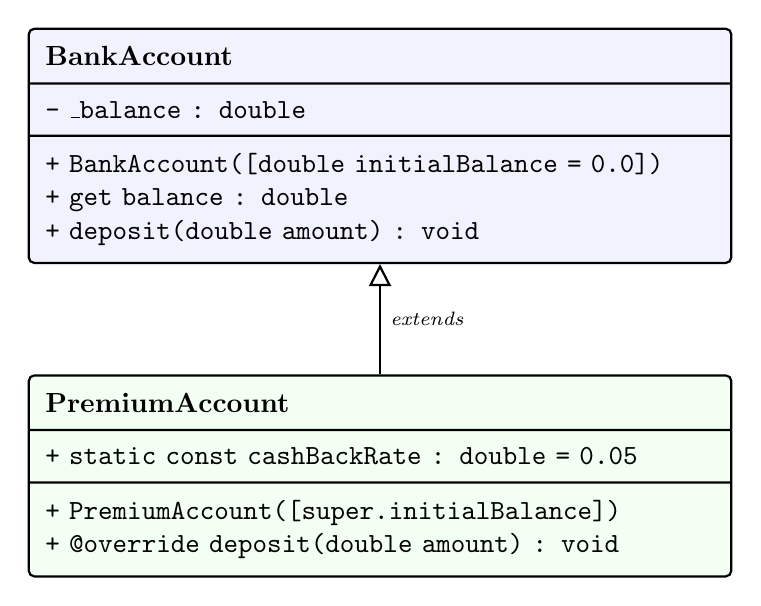
\begin{tikzpicture}[
    classbox/.style={
        rectangle split, 
        rectangle split parts=3, 
        draw=black, 
        thick, 
        fill=blue!5, 
        rounded corners=2pt, 
        text width=8.5cm, 
        inner sep=6pt, 
        align=left
    },
    arrow/.style={-{Triangle[open, length=8pt, width=8pt]}, thick}
]

% Base Class: BankAccount
\node[classbox] (BankAccount) {
    \textbf{\centering BankAccount}
    \nodepart{second}
    \texttt{- \_balance : double}
    \nodepart{third}
    \texttt{+ BankAccount([double initialBalance = 0.0])}\\
    \texttt{+ get balance : double}\\
    \texttt{+ deposit(double amount) : void}
};

% Sub Class: PremiumAccount
\node[classbox, below=1.4cm of BankAccount, fill=green!5] (PremiumAccount) {
    \textbf{\centering PremiumAccount}
    \nodepart{second}
    \texttt{+ static const cashBackRate : double = 0.05}
    \nodepart{third}
    \texttt{+ PremiumAccount([super.initialBalance])}\\
    \texttt{+ @override deposit(double amount) : void}
};

% Inheritance Arrow
\draw[arrow] (PremiumAccount.north) -- node[right, font=\scriptsize\itshape] {extends} (BankAccount.south);

\end{tikzpicture}
\captionof{figure}{UML Class Diagram of the Digital Wallet Backend}
\end{center}

\vspace{0.2cm}

% ==============================================================================
% PAGE 3: MATHEMATICAL FORMULATION & EXPERIMENTAL VERIFICATION
% ==============================================================================
\section*{3. Mathematical Formulation of Account Transactions}
\noindent\rule{\textwidth}{0.5pt}\vspace{0.08cm}

For any transaction requesting a deposit of monetary amount $A \in \mathbb{R}^+$, the state transition is governed by the account tier:

\begin{enumerate}
    \setlength{\itemsep}{4pt}
    \item \textbf{Standard Account Credit Equation:}
    \begin{equation}
        B_{t+1} = B_t + A, \quad \text{subject to } A > 0
    \end{equation}
    where $B_t$ represents the current encapsulated balance and $B_{t+1}$ denotes the post-transaction balance.

    \item \textbf{Premium Account Credit Equation with 5\% Cash-Back:}
    Let $r = 0.05$ represent the invariant cash-back bonus reward rate. The earned reward bonus $R(A)$ and effective credited amount $C_{\text{eff}}(A)$ are:
    \begin{equation}
        R(A) = A \times r = 0.05 \cdot A
    \end{equation}
    \begin{equation}
        C_{\text{eff}}(A) = A + R(A) = A \cdot (1 + r) = 1.05 \cdot A
    \end{equation}
    The resulting balance state transition is consequently formulated as:
    \begin{equation}
        B_{t+1} = B_t + C_{\text{eff}}(A) = B_t + 1.05 \cdot A, \quad \text{subject to } A > 0
    \end{equation}
\end{enumerate}

\vspace{0.15cm}
\section*{4. Experimental Verification and Results}
\noindent\rule{\textwidth}{0.5pt}\vspace{0.1cm}

The system implementation was subjected to comprehensive test suites covering initialization, deposit accuracy, cash-back reward verification, polymorphic dynamic dispatch, and boundary condition rejection:

\vspace{0.12cm}
\begin{center}
\begin{tabular}{llcccc}
\toprule
\textbf{Scenario} & \textbf{Account Type} & \textbf{Initial (\$)} & \textbf{Deposit (\$)} & \textbf{Bonus (\$)} & \textbf{Final Balance (\$)} \\
\midrule
1. Standard Deposit 1 & \texttt{BankAccount} & 100.00 & 500.00 & 0.00 & 600.00 \\
1. Standard Deposit 2 & \texttt{BankAccount} & 600.00 & 250.00 & 0.00 & 850.00 \\
\midrule
2. Premium Deposit 1 & \texttt{PremiumAccount} & 100.00 & 500.00 & 25.00 (+5\%) & 625.00 \\
2. Premium Deposit 2 & \texttt{PremiumAccount} & 625.00 & 1000.00 & 50.00 (+5\%) & 1675.00 \\
\midrule
3. Polymorphic Batch \#1 & \texttt{BankAccount} & 200.00 & 400.00 & 0.00 & 600.00 \\
3. Polymorphic Batch \#2 & \texttt{PremiumAccount} & 200.00 & 400.00 & 20.00 (+5\%) & 620.00 \\
\midrule
4. Invalid Input Check & \texttt{BankAccount} & 850.00 & 0.00 & Rejected & 850.00 (Unchanged) \\
4. Negative Input Check & \texttt{PremiumAccount} & 1675.00 & -75.00 & Rejected & 1675.00 (Unchanged) \\
\bottomrule
\end{tabular}
\captionof{table}{Experimental Test Scenarios and Quantitative Transaction Ledger}
\end{center}

\vspace{0.18cm}
\subsection*{4.1 Terminal Execution Log}
\begin{lstlisting}[language=bash, basicstyle=\ttfamily\scriptsize, frame=single, backgroundcolor=\color{black!5}]
======================================================================
        DIGITAL WALLET BACKEND SYSTEM - TEST & VERIFICATION           
======================================================================

--- Scenario 1: Standard Account (Encapsulation & Deposit) ---
Initial Balance (via getter): $100.00
Performing deposits:
  [Deposit] Credited: $500.00 | Current Balance: $600.00
  [Deposit] Credited: $250.00 | Current Balance: $850.00
Final Standard Account Balance: $850.00

--- Scenario 2: Premium Account (Inheritance & 5% Cash-Back) ---
Initial Balance (via getter): $100.00
Performing deposits (eligible for 5% reward):
  [Premium Reward] 5% Cash-Back Bonus: +$25.00 (Base: $500.00)
  [Deposit] Credited: $525.00 | Current Balance: $625.00
  [Premium Reward] 5% Cash-Back Bonus: +$50.00 (Base: $1000.00)
  [Deposit] Credited: $1050.00 | Current Balance: $1675.00
Final Premium Account Balance: $1675.00

--- Scenario 3: Polymorphism (Heterogeneous Collection) ---
Processing Account #1 [Type: BankAccount]:
  Opening Balance: $200.00
  [Deposit] Credited: $400.00 | Current Balance: $600.00
  Closing Balance: $600.00

Processing Account #2 [Type: PremiumAccount]:
  Opening Balance: $200.00
  [Premium Reward] 5% Cash-Back Bonus: +$20.00 (Base: $400.00)
  [Deposit] Credited: $420.00 | Current Balance: $620.00
  Closing Balance: $620.00

--- Scenario 4: Input Validation & Boundary Edge Cases ---
Attempting zero deposit on Standard Account:
  [Error] Invalid deposit: $0.00. Amount must be greater than zero.
Attempting negative deposit on Premium Account:
  [Error] Invalid deposit: $-75.00. Amount must be greater than zero.

======================================================================
                 ALL VERIFICATION TESTS COMPLETED                     
======================================================================
\end{lstlisting}

\newpage

% ==============================================================================
% PAGE 4: DISCUSSION & CONCLUSION
% ==============================================================================
\section*{5. Discussion and Architectural Evaluation}
\noindent\rule{\textwidth}{0.5pt}\vspace{0.1cm}

\begin{itemize}
    \setlength{\itemsep}{3.5pt}
    \item \textbf{Integrity Guarantees via Encapsulation:} Financial backends demand zero-tolerance for unintended balance corruption. By encapsulating \texttt{\_balance} and only exposing a read-only getter, the class guarantees that external client code cannot assign arbitrary values. Every mutation is routed strictly through \texttt{deposit()}, ensuring that transaction validation rules (e.g., $A > 0$) are unfailingly applied.
    \item \textbf{Extensibility through Inheritance:} The addition of \texttt{PremiumAccount} required zero modifications to existing \texttt{BankAccount} core logic, adhering to the \textit{Open-Closed Principle} (open for extension, closed for modification). Subclasses can introduce distinct business models (e.g., Student accounts, Merchant wallets) with minimal boilerplate.
    \item \textbf{Polymorphic Code Decoupling:} As evidenced in Scenario 3, iterating over a collection of \texttt{List<BankAccount>} enabled batch transaction processing without explicit conditional branching (\texttt{if (account is PremiumAccount)}). The Dart Virtual Machine accurately dispatched the correct overridden \texttt{deposit()} method, promoting clean and decoupled architectural design.
    \item \textbf{Relevance to IoT Edge Platforms:} In IoT edge computing and connected payment terminal applications (such as automated transit kiosks or smart metering systems), modular digital wallet backends ensure secure offline balance tracking, verified reward distributions, and maintainable embedded codebases.
\end{itemize}

\vspace{0.25cm}
\section*{6. Conclusion}
\noindent\rule{\textwidth}{0.5pt}\vspace{0.1cm}

All architectural objectives stipulated in the laboratory requirements were rigorously implemented, executed, and verified:
\begin{enumerate}
    \setlength{\itemsep}{2pt}
    \item The base \texttt{BankAccount} class successfully protects internal state via library privacy and exposes controlled getter inspection.
    \item The derived \texttt{PremiumAccount} class cleanly overrides \texttt{deposit()} to automatically credit an accurate 5\% cash-back reward bonus.
    \item Subtype polymorphism guarantees seamless interoperability across heterogeneous account collections.
    \item Edge validation ensures resilience against invalid non-positive deposit attempts.
\end{enumerate}

\newpage

% ==============================================================================
% PAGE 5: DART SOURCE CODE LISTING
% ==============================================================================
\section*{7. Complete Dart Source Code Listing (\texttt{digital\_wallet.dart})}
\noindent\rule{\textwidth}{0.5pt}\vspace{0.15cm}

\noindent\textbf{GitHub File Link:}\\
\href{https://github.com/Masud744/flutter-lab/blob/main/Lab_01/src/digital_wallet.dart}{\texttt{https://github.com/Masud744/flutter-lab/blob/main/Lab\_01/src/digital\_wallet.dart}}\vspace{0.2cm}

\lstinputlisting[language=Dart]{../src/digital_wallet.dart}

\end{document}
